% Chapter Template

\chapter{Supervised Sequence Learning} % Main chapter title

\label{Chapter2} % Change X to a consecutive number; for referencing this chapter elsewhere, use \ref{ChapterX}

\lhead{Chapter 2. \emph{Supervised Sequence Learning}} % Change X to a consecutive number; this is for the header on each page - perhaps a shortened title

%----------------------------------------------------------------------------------------
%	SECTION 1
%----------------------------------------------------------------------------------------

\emph{In this chapter we present the state-of-the-art technique for metadata extraction, conditional random fields (CRF). For completeness, we include a background history of related machine learning techniques and their associated optimisation algorithms. We begin with a presentation of Hidden Markov Models (HMM) and their inference algorithms. Following this we present multinomial logistic regression. From these former topics we show how their ideas are combined to produce Maximum Entropy Markov Models (MEMM) and CRFs. Notably, we pinpoint the part of the mathematical model relevant to our work on feature engineering. Finally, we describe Wapiti, a general-purpose software engine for training and applying CRF models.}

\section{Hidden Markov Models}

Hidden Markov models (HMMs) are a staple of natural language processing (NLP) and other engineering fields. A HMM models a probability distribution over an unknown, ``hidden'' sequence state variables of length $T$, $\mathbf{y} = (y_1, y_2, ..., y_T)$, whose elements take on values in a finite set of states, S, and follow a Markov process. For each element in this hidden sequence, there is a corresponding observation element, forming a sequence of \emph{observations}, $\mathbf{x} = (x_1, x_2, ..., x_T)$, similarly taking values in a finite set, O. The graphical structure of an HMM (Figure \ref{fig:HMM}) shows the dependencies between consecutive hidden states (these are modelled with \emph{transition} probabilities), and states and their observations (modelled with \emph{emission} probabilities). The first dependency is referred to as the Markov condition, which postulates the dependency of each hidden state, $y_t$, on its k precursors in the hidden sequence, namely, $\mathbf{y}_{t-k:t-1}$\footnote{In the following we use the notation $\mathbf{x}_{a:b}$ to refer to the the subsequence of vector $\mathbf{x}$ from index $a$ through $b$ inclusive.}. In the discussion that follows, we assume the Markov condition to be of first degree, that is, $k =1$. Incidentally, higher-order HMMs may always be reconstructed to this simplest form\cite{reference}. The second dependency may be referred to as \emph{limited lexical conditioning}, referring to the dependency of an observation only on its hidden state. Properties of the model may then be deduced through statistical inference, for example a prediction of the the most likely hidden sequence can be computed with the Viterbi algorithm (section \ref{subsec:viterbi}).

HMMs have been shown to be successful in statistical modelling problems. In Part of Speech (PoS) tagging, a classic NLP problem for disambiguating natural language, the parts of speech (nouns, verbs, and so on) of a word sequence (sentence) are modelled as hidden states, and the words themselves are the observations. The PoS sequence may be modelled and predicted using n HMM. Even a simple HMM can achieve an accuracy of well over $90\%$. The problem of metadata extraction is clearly similar in form to PoS tagging, as we further show in section \ref{sec:ame}.

\begin{figure}[!ht]
\center
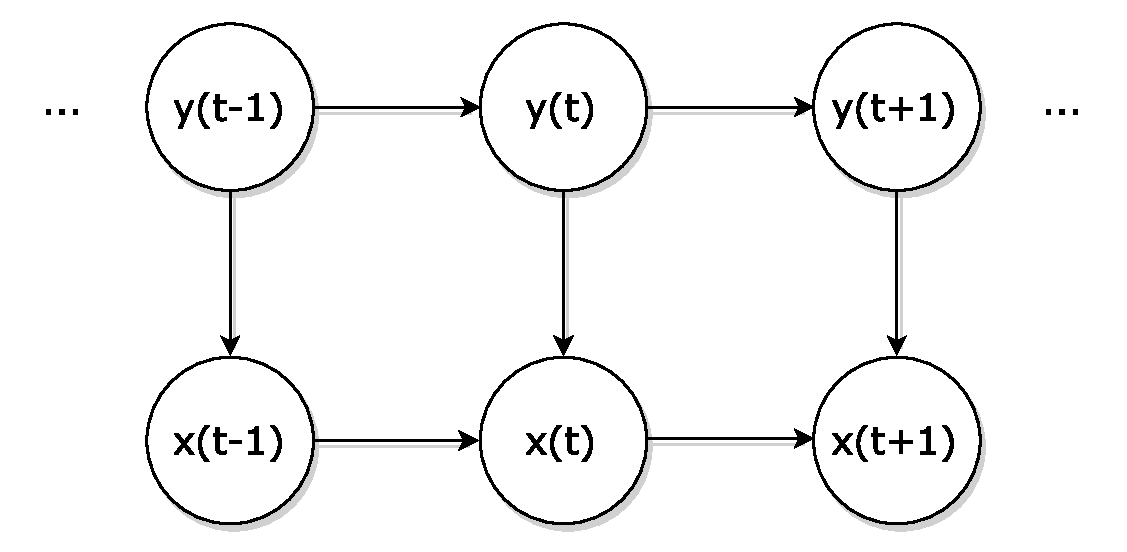
\includegraphics[width=4in]{Figures/HMM.pdf}
\caption{An Illustration of the graphical structure of a Hidden Markov Model (HMM). The arrows indicate the dependencies running from dependent to dependee.}
\label{fig:HMM}
\end{figure}

We may build a HMM by first forming the joint probability distribution of the hidden state sequence and the observation sequence,

\begin{equation}
\p(\mathbf{x}, \mathbf{y}) = \p(\mathbf{x} | \mathbf{y}) \p(\mathbf{y}).
\label{eq:joint}
\end{equation}

Applying the chain rule and the dependency assumptions, we acquire,

\begin{equation}
\begin{aligned}
\p(\mathbf{x} | \mathbf{y}) &= \p(x_1|\mathbf{y}) \p(x_2|x_1, \mathbf{y}) ... \p(x_T|\mathbf{x}_{1:T-1}\mathbf{y}) \\
&= \p(x_1|y_1) \p(x_2|y_2) ... \p(x_T|y_T),
\end{aligned}
\label{eq:conditional}
\end{equation}

and,

\begin{equation}
\begin{aligned}
\p(\mathbf{y}) &= \p(y_1) \p(y_2|y_1) ... \p(y_T, \mathbf{y}_{1:T-1}) \\
&= \p(y_1) \p(y_2|y_1) ... \p(y_T, y_{T-1}).
\end{aligned}
\label{eq:prior}
\end{equation}

Thus, we may rewrite the factorisation of the HMM as,

\begin{equation}
\p(\mathbf{x}, \mathbf{y}) = \prod_{t=1}^T p(y_t | y_{t-1})p(x_t | y_t)
\label{eq:factorisedHMM}
\end{equation}

The probabilities $p(y_t | y_{t-1})$ are known as \emph{transition} probabilities, and $p(x_t | y_t) $ as \emph{emission} probabilities. These probabilities constitute the model parameters, $\theta = (\mathbf{A}, \mathbf{B}, \mathbf{I})$, where $\mathbf{A}$ is the $|S| \times |S|$ matrix of probabilities of transitioning from one state to another, $\mathbf{B}$ is the $|S| \times |O|$ matrix of probabilities of emitting an observation given an underlying hidden state, and $\mathbf{I}$ is the vector of probabilities of initial states. The model parameters must be precomputed\footnote{For example, the model parameters can be estimated through application of the Baum-Welch algorithm on an unsupervised training set.}. Now, given a sequence of observations, $\textbf{x}$, we may predict the hidden state sequence, $\mathbf{y}*$, by maximising the conditional distribution, $\p(\mathbf{y} | \mathbf{x})$. Thus,

\begin{equation}
\textbf{y}* = \argmax_{\textbf{y}}\Bigg\{\prod_{t=1}^T p(y_t | y_{t-1})p(x_t | y_t)\Bigg\}.
\label{eq:argmax}
\end{equation}

The hidden state sequence prediction is chosen to be the one maximising the likelihood over all possible hidden sequences. This seemingly intractable problem may be solved in polynomial time using dynamic programming (see section \ref{subsec:viterbi}).

\subsection{Viterbi Algorithm}
\label{subsec:viterbi}

The Viterbi algorithm is used to efficiently compute the most likely sequence, $\textbf{y}$, given an observation sequence, $\textbf{x}$. The algorithm can do this efficiently by working along the sequence from state to state, and choosing the transitions that maximise the likelihood of the sequence fragment. To show this we define, $v_t(s) = \max_{\mathbf{y}_{1:t-1}} \p(\mathbf{y}_{1:t-1}, y_t = s | \mathbf{x})$, that is, the most likely sequence from the first $t-1$ states, with the choice of state $s$ at time $t$. Thus, we may write,

\begin{equation}
\begin{aligned}
v_t(s) &= \max_{\mathbf{y}_{1:t-1}} \p(\mathbf{y}_{1:t-1} | \mathbf{x}) \p(y_{t-1}, y_t = s) \p(x_t | y_t = s) \\
&= \max_{\mathbf{y}_{1:t-1}} v_{t-1}(y_{t-1}) \p(y_{t-1}, y_t = s) \p(x_t | y_t = s), 
\end{aligned}
\label{eq:viterbi}
\end{equation}

and we may see the recursion. Once all states have been computed at time $t$, the maximum may be chosen and the algorithm proceeds to time $t+1$. Pseudocode for the Viterbi algorithm is given in Algorithm \ref{alg:viterbi} in \ref{sec:appendix}. The algorithm must test all $|S|$ transitions from the previous state to each of the $|S|$ current states, and it does that for each of the $|T|$ steps in the sequence. Hence the complexity of the algorithm is a workable $\mathcal{O}(T|S|^2)$.

\section{Forward-backward Algorithm}
\label{sec:fb}

Another key algorithm to sequence learning is the forward-backward algorithm, so called for its computation of variables in both directions along the sequence. It is another example of a dynamic programming algorithm and is used to compute the so-called \emph{forward-backward} variables, which are the conditional probabilities of the individual hidden states at each time step (that is, not the whole sequence), given the observation sequence and model parameters, namely, $\p(y_t = s | \mathbf{x}, \theta)$. These conditional probabilities have many useful applications, for example in the Baum-Welch algorithm for estimating model parameters, but also for in the training of \emph{conditional random fields}, as we show in section \ref{subsec:crfs}. We may write the forward-backward variables as,

\begin{equation}
\gamma_t(s) = \p(y_t = s | \mathbf{x}, \theta) = \frac{\alpha_t(s) \beta_t(s)}{\sum_{s' \in S} \alpha_t(s') \beta_t(s')},
\label{eq:fb}
\end{equation}

where the \emph{forward} variables, $\alpha_t(s) = \p(\mathbf{x}_{t+1:n}|y_t = s, \mathbf{x}_{1:t}) = \p(\mathbf{x}_{t+1:n}|y_t = s)$, and the \emph{backward} variables, $\beta_t(s) = \p(y_t = s, \mathbf{x}_{1:t})$. To derive the forward-backward algorithm we write, by the law of total probability,

\begin{equation}
\begin{aligned}
\alpha_t(s) &= \sum_{y_{t-1}} \p(y_{t-1}, y_t = s, \mathbf{x}_{1:t}) \\
& = \sum_{y_{t-1}} \p(y_t = s|y_{t-1}) \p(x_t|y_t) \p(y_{t-1}, \mathbf{x}_{1:t-1}) \\
& = \sum_{y_{t-1}} \mathbf{A}(y_{t-1}, s) \mathbf{B}(x_t, y_t) \alpha_{t-1}(y_{t-1})).
\end{aligned}
\label{eq:forward}
\end{equation}

Thus, we may see the recursion, as well as the way the forward variables will be computed, traversing the sequence in the forward direction with each forward variable of a given time a weighted product of those from the previous time. Likewise, for the backward variables, we may write,

\begin{equation}
\begin{aligned}
\beta_t(s) &= \sum_{y_{t+1}} \p(y_t = s, y_{t+1}, \mathbf{x}_{t+1:n}) \\
& = \sum_{y_{t+1}} \p(\mathbf{x}_{t+2:n}|y_{t+1}, x_{t+1}) \p(x_{t+1}, y_{t+1}|y_t = s) \\
& = \sum_{y_{t+1}} \beta_{t+1}(y_{t+1}) \mathbf{A}(s, y_{t+1}) \mathbf{B}(x_{t+1}, y_{t+1})).
\end{aligned}
\label{eq:backward}
\end{equation}

From equations \ref{eq:forward} and \ref{eq:backward} comes Algorithm \ref{alg:fb}. The complexity of the algorithm comes from noting that at each of the $T$ steps in the sequence (in either direction), we compute $|S|$ variables, involving a summation of $|S|$ products. Hence, like the Viterbi algorithm, the complexity of the forward-backward algorithm is $\mathcal{O}(T|S|^2)$.

\section{Maximum Entropy Classifiers}

Maximum entropy classifiers, also known as multinomial logistic regression, are a family of classification techniques.  A prediction is a discrete (categorical), scalar \emph{class}, rather than a class sequence as it is for HMMs. To build a model, we require a \emph{training set} consisting of a $N \times D$ matrix, $\mathbf{X}$, of $N$ training samples of dimension $D$\footnote{The dimensions of a model is synonymous with the model fields or features.}, as well as the $N$ corresponding classifications in the form of a vector, $\mathbf{y}$. A convex cost function known as a maximum log-likelihood function is constructed and subsequently optimised over the choice of model parameters, denoted $\beta$. Thus, building a model is equivalent to solving a convex optimisation problem. A classification (prediction), $y*$, for an unseen data sample, $\mathbf{x}$, is made by applying these optimal model parameters linearly. The result is then passed through a non-linear \emph{logistic} function, denoted $\sigma$ to obtain a probability. Formally,

\begin{equation}
y* = \sigma(\beta^T\mathbf{x}).
\label{eq:logisticprediction}
\end{equation}

The simplest form of maximum entropy classifier is binary logistic regression, where the number of classes to predict from is two, denoted $C_1$ and $C_2$. In this case, $\p(y_n = C_1|\mathbf{x}_n;\beta) = \sigma(\beta^T\mathbf{x}_n)$, and $\p(y_n = C_2|\mathbf{x}_n;\beta) = 1 - \sigma(\beta^T\mathbf{x}_n)$, where $C_1$ and $C_2$ are encoded as 0 and 1 respectively. Notice the probabilities sum to 1. Now, the log-likelihood can be expressed as,

\begin{equation}
\begin{aligned}
\log\p(\mathbf{y}|\mathbf{X}, \boldsymbol\beta) = \log\prod_{n=1}^N \p(y_n, \mathbf{x}_n)
&= \log\Bigg(\prod_{n:y_n = C_1}^N \sigma(\beta^T\mathbf{x}_n) \prod_{n:y_n = C_2}^N 1 - \sigma(\beta^T\mathbf{x}_n)\Bigg) \\
&=  \log\prod_{n = 1}^N \sigma(\beta^T\mathbf{x}_n)^{y_i}(1 - \sigma(\beta^T\mathbf{x}_n))^{1 - y_i}
\end{aligned}
\label{eq:logistic2}
\end{equation}

where $y_i \in \{0, 1\}$. We may then generalise to,

\begin{equation}
\begin{aligned}
\log\p(\mathbf{y}|\mathbf{X}, \boldsymbol\beta) = \log \prod_{n = 1}^N \prod_{c = 1}^C \mu_{ic}^{y_{ic}},
\end{aligned}
\label{eq:multinomial}
\end{equation}

where $y_{ic} = \mathbbm{1}_{y_i = c}$ and $y_i$ is a bit vector indicating the class of the $i$th sample. In this general, multinomial case, the probabilities are written, $\mu_{ic} = \frac{\exp(\beta_c^T\mathbf{x}_i)}{\sum_{c' = 1}^C \exp(\beta_c^T\mathbf{x}_i)}$, which are normalised to ensure they sum to 1, and $\beta_c$ is part of a set of $C$ parameter vectors notated as $D \times C$ matrix, $\mathbf{B}$. From this we obtain a cost function,

\begin{equation}
\mathcal{L}(\mathbf{B}) = 
\log\p(\mathbf{y}|\mathbf{X}, \mathbf{B}) = \sum_{n=1}^N  \Bigg( \sum_{c = 1}^C y_{ic}\beta_c^T \mathbf{x}_n \Bigg) - \log \Bigg( \sum_{c' = 1}^C \exp(\beta_{c'}^T\mathbf{x}_n) \Bigg).
\label{eq:logisticcost}
\end{equation}

We then require an optimisation algorithm to solve for $\mathbf{B}$.

\section{L-BFGS}
\label{sec:lbfgs}

Convex optimisation problems may be solved numerically using variants of the method of greatest descent. These methods find the optimal model parameters by iteratively approaching the global minimum cost by taking steps along the cost function hypersurface opposite to the gradient. The classic first-order gradient descent algorithm defines its iteration step to be,

\begin{equation}
\boldsymbol\beta^{k+1} = \boldsymbol\beta^{k} - \alpha\nabla\mathcal{L}(\boldsymbol\beta^{k}),
\label{eq:gd}
\end{equation}

where $\beta$ is the vector of model parameters, $\alpha$ is the step size, and $\mathcal{L}$ is the cost function. Newton's method (also known as Iterated Reweighted Least Squares, IRLS) takes a step in the direction minimising a second-order approximation of the cost function,

\begin{equation}
\boldsymbol\beta^{k+1} = \boldsymbol\beta^{k} - \alpha_k \mathbf{H_k}^{-1}\nabla\mathcal{L}(\boldsymbol\beta^{k}),
\label{eq:newton}
\end{equation}

where $\mathbf{H}$ is the $(D \times D)$ Hessian matrix of partial second derivatives. For smaller problems, these algorithms are adequate, however for models with millions of features, such as those that may be encountered in metadata extraction, smarter approaches are required. The \emph{Broyden--Fletcher--Goldfarb--Shanno} (BFGS) algorithm saves on the expensive computation of the Hessian by building up an approximation iteratively. The \emph{limited memory} BFGS (L-BFGS) algorithm makes further savings on the Hessian's \emph{storage}, and has come to be the standard learning algorithm for such problems. The L-BFGS algorithm is the tool of choice for many problems\cite{murphy2012machine} and is the algorithm we use in our analysis.

\section{Regularisation}

To avoid overfitting, we add a penalty to the cost function. This imposes a cost proportional to the size of the parameters for each dimension. Large parameters are therefore discouraged and helps prevent the creation of complex models during training which do not fit test data well. This is equivalent to adding model constraints to the convex optimisation problem. The two most common regularisation types are known as $l_1$ ad $l_2$ regularisation. The former imposes a \emph{Laplace} prior distribution on the parameters, and the latter a \emph{Gaussian}\footnote{A prior distribution in the Bayesian sense is the initial distribution of a variable taken independently.}. In a probabilistic interpretation, this makes large parameters less likely and moderates their choices, and this is expressed in the cost function as the penalty. In our work, $l_2$ is the only type of regularisation compatible with L-BFGS (section \ref{subsec:lbfgs}).

\section{Conditional Random Fields}
\label{subsec:crfs}

Conditional Random Fields (CRFs) are a machine learning technique for making structured predictions. They are an improvement to the similar, Maximum Entropy Markov models (MEMM)\cite{mccallum2000maximum}, which combine aspects of maximum entropy classifiers and Hidden Markov models.\cite{lafferty2001conditional}. They are a member of a class of structured sequence models called \emph{random fields}, which are part of a broader family known as \emph{graphical models}, including within it \emph{Bayesian networks}.

Classification over relational data can benefit greatly from rich features, that is, describing observed attributes of an observation beyond merely its identity (as with HMMs). For example, in the context of text processing, we might consider describing a string token (observation) by non-lexical features such as by its capitalisation or punctuation. Furthermore, we may wish to model context-aware features that contrast a string token with its surroundings. However, the complexity of the interdependencies of such features will likely make their explicit modelling infeasible. With CRFs, we circumvent this problem by instead modelling the conditional distribution $p(\mathbf{y}|\mathbf{x})$ of the underlying graph structure, giving us a free choice over features and, in so doing, \emph{implicitly} defining a distribution over $\mathbf{x}$ without having to model this distribution directly.\cite{sutton2006introduction}. Such a conditional model is called a \emph{discriminative} model, in contrast to a \emph{generative} model, whereby the joint probability distribution is modelled explicitly. If we wish to model the interdependencies in a generative model, we must either extend the model (which may be difficult) and entail intractable solution algorithms, or we must simplify the model and thereby compromise model performance. Notice that modelling the conditional distribution is sufficient for classification, wherein the observation sequence is known. This freedom for rich feature engineering is what make CRFs the current state of the art in metadata extraction, where arbitrarily defined features often make for good indicators. One may be tempted to use a logistic regression and classify each part of a sequence separately, but this would fail to take into account the contextual relations between the entities. For example in the metadata extraction of a bibiographic reference, it is more likely for a publication title to follow an author list, and for a journal name to follow a publication title. This is what we mean by structured sequence learning, where the data to predict exhibits interdependencies and are correlated.

When the graph structure of the CRF model is the same as for a HMM (Figure \ref{fig:HMM}), we have what is called a \emph{linear-chain} CRF. HMMs and linear-chain CRFs form what is called a generative-discriminative pair. In the general case, where the graph structure is more complex, we have what is called \emph{skip-chain} CRFs. In this case the problem becomes far more complex, and we will not discuss general CRFs here. A HMM may alternatively be expressed by the joint probability,

% \begin{equation}
% p(\textbf{x}, \textbf{y}) = \text{exp} \Bigg\{\sum_t{
% \sum_{i, j \in S}{
% \lambda_{ij}\mathbbm{1}_{\{y_t = i\}}\mathbbm{1}_{\{y_{t-1} = j\}}
% }
% + \sum_t\sum_{i \in S}\sum_{o \in O}{
% \mu_{io}\mathbbm{1}_{\{y_t = i\}}\mathbbm{1}_{\{x_t = o\}}
% }
% }\Bigg\},
% \label{eq:jointcrf}
% \end{equation}

\begin{equation}
p(\textbf{x}, \textbf{y}) = \text{exp} \Bigg\{
\sum_{i, j \in S}{
\lambda_{ij}F_{i,j}(y_t, y_{t-1}, x_t)
}
+
\sum_{i \in S}\sum_{o \in O}{
\mu_{io}F_{i,o}(y_t, y_{t-1}, x_t)
}
\Bigg\},
\label{eq:jointcrf}
\end{equation}

where $\lambda_{ij}$ are the transition probabilities and $\mu_{ij}$ are the emission probabilities. $F_{i,j}(y_t, y_{t-1}, x_t) = \sum_t^T\mathbbm{1}_{\{y_t = i\}}\mathbbm{1}_{\{y_{t-1} = j\}}$ is a \emph{feature function} used to activate the transition probabilities, and $F_{i,o}(y_t, y_{t-1}, x_t) = \sum_t^T\mathbbm{1}_{\{y_t = i\}}\mathbbm{1}_{\{x_{i} = o\}}$ for the emissions. The indicator functions activate the probabilities in accordance with the identity of the states and observations. Regardless, this formulation is equivalent to \ref{eq:factorisedHMM}. With some notational abuse we can define the more compact expression,

\begin{equation}
\p(\textbf{x}, \textbf{y}) = \text{exp} \Bigg\{\sum_k{
\lambda_{k}F_{k}(y_t, y_{t-1}, x_t)
}\Bigg\}.
\label{eq:jointcrfcompact}
\end{equation}

Where $F_k$ is a general feature function and $\lambda_k$ a general feature weight. Now we may define the discriminative counterpart to this joint distribution; the linear-chain CRF,

\begin{equation}
p(\textbf{y}|\textbf{x}) = \frac{p(\textbf{x}, \textbf{y})}{\sum_{y'}{p(\textbf{x}, \textbf{y}')}} = \frac{1}{Z(\mathbf{x})}\exp \Bigg\{\sum_k{
\lambda_{k}F_{k}(y_t, y_{t-1}, x_t)
}\Bigg\},
\end{equation}

where $Z(\mathbf{x}) = \sum_{y'}\exp \Big\{\sum_k{\lambda_{ij}F_{k}(y'_t, y'_{t-1}, x_t)}\Big\}$ is known as the partition function, ensuring probabilities sum to 1. Whereas HMMs model only the \emph{occurence} of a word, with conditional random fields we may choose $F_k$ to define arbitrarily complex features, describing rich information about a word, its attributes, and its context. Finally, we may define a cost function in the following way,

\begin{equation}
l(\theta) = \sum_{i=1}^N\sum_{t=1}^T\sum_{k=1}^K\lambda_kF_{k}(y_t, y_{t-1}, x_t) - \sum_{i=1}^N\log Z(\mathbf{x}^{(i)}) - \sum_{k=1}^K \frac{\lambda_k^2}{2\sigma^2},
\end{equation}

where $\theta = \{\lambda_k\}_{k=1}^K$. This is called penalised maximum log likelihood. The penalty term, $\sum_{k=1}^K\frac{\lambda_k^2}{2\sigma^2}$, imposes an $l_2$ regularisation on the solution parameters, $\lambda_k$. However, according to McCallum et al. (2004), varying the tuning parameter, $\sigma^2$ (the variance), by orders of magnitude has little effect on the outcome\cite{mccallum}, a claim we corroborate in section \ref{sec:results}. This cost function represents a strictly convex function, solvable using numerical methods such as L-BFGS (see section \ref{sec:lbfgs}). Forward-backward processing (section \ref{sec:fb}) is performed at each iteration to compute the partition function, as well as the conditional probabilities resulting from forming the partial derivatives required for gradient descent. Finally, the Viterbi algorithm (section \ref{subsec:viterbi}) is used to make a prediction with the trained model, that is, the best state sequence is found given the optimal parameter set found in training. A detailed exposition of this is given in \cite{Mccallum}.

\section{Feature Functions}
\label{sec:featurefunctions}

In the simple HMM case (equation \ref{eq:jointcrf}), there is a single feature function for each $(i, j)$ and $(i, o)$ pair. Furthermore, they are merely indicator functions that facilitate the activation of the transition and emission probabilities. In CRFs, however, we may define arbitrarily many and varied feature functions of the form $F_k(\mathbf{x}, y) = \sum_t^T f_k(\mathbf{x}, y)$, where $f_k$ is a (typically boolean) function describing one of several features about a token. Notice that while such a function is centered on a given token, that is, a specific element of $\mathbf{x}$, the function has access to the full vector $\mathbf{x}$, enabling the creation of context-aware features, combining information about a tokens with its neighbours. Further notice that the summation over the sequence is what enables instances (token sequences) of varying lengths to remain compatible with the model.

The form of the functions themselves, $f(\cdot)$, are known in Wapiti (section \ref{sec:wapiti}) as \emph{templates}. It is in choosing these explicitly that we perform feature engineering. The literal feature functions, $\{f_k\}_{k=1}^K$, are formed by resolving the templates over the \emph{vocabularly} of features encountered in the extraction process prior to model training. In this way, we may see how model complexity depends on the diversity of the training set, and consequently, for smaller training sets, a model will have fewer feature functions. 

\section{Wapiti}
\label{sec:wapiti}

There are several open source softwares for the general purpose training and application of conditional random fields and related models. Wapiti is the tool of choice for this project, given its compatibility with metadata extraction tool GROBID (section \ref{sec:grobid}), its speed advantage over alternatives, and its recency of its development. It is developed by Thomas Lavergne at LIMSI, a computer science laboratory in Orsay affiliated with Paris-Sud University.

[Here some information about Wapiti's capabilities] parallelisable

INCLUDE CITATION OF WAPITI

Wapiti's main functions are training models and tagging. Training requires two inputs:

\begin{enumerate}
\item a feature template file, and;
\item a file of extracted features.
\end{enumerate}

The output of training is a model file. Tagging requires three inputs:

\begin{enumerate}
\item a feature template file;
\item a file of extracted features, and;
\item a trained model.
\end{enumerate}

The output of tagging is the file of extraction features appended with the classifications of each token.

\subsection{Feature Templates}

Feature templates are the main access point for modelling with Wapiti. These files use a special syntax introduced by an older CRF engine, \emph{CRF++} (also supported by GROBID), allowing the operator to specify the form of the feature functions to be implemented in the model (see Section \ref{sec:featurefunctions}). The features are listed in a manner such as seen in Figure \ref{fig:featuretemplatefile}.

\begin{figure}
\begin{verbatim}
* Initialize the model
* Summary
    nb train:    493
    nb labels:   7
    nb blocks:   5816
    nb features: 40754
* Train the model with l-bfgs
  [   1] obj=1688,58    act=16482    err=25,80%/50,91% time=0,08s/0,08s
  [   2] obj=1221,30    act=15580    err=19,11%/35,50% time=0,05s/0,12s
  [   3] obj=922,15     act=13869    err=17,20%/33,67% time=0,04s/0,17s
  [   4] obj=638,04     act=10845    err= 6,53%/15,21% time=0,04s/0,20s
  [   5] obj=478,72     act=10582    err= 5,68%/13,59% time=0,04s/0,24s
  [   6] obj=416,15     act=9926     err= 3,77%/ 9,53% time=0,04s/0,28s
\end{verbatim}
\caption{Output from training date model}
\label{fig:featuretemplatefile}
\end{figure}


\subsection{Extracted Features}

\subsection{Models}


\begin{figure}
\begin{verbatim}
* Initialize the model
* Summary
    nb train:    493
    nb labels:   7
    nb blocks:   5816
    nb features: 40754
* Train the model with l-bfgs
  [   1] obj=1688,58    act=16482    err=25,80%/50,91% time=0,08s/0,08s
  [   2] obj=1221,30    act=15580    err=19,11%/35,50% time=0,05s/0,12s
  [   3] obj=922,15     act=13869    err=17,20%/33,67% time=0,04s/0,17s
  [   4] obj=638,04     act=10845    err= 6,53%/15,21% time=0,04s/0,20s
  [   5] obj=478,72     act=10582    err= 5,68%/13,59% time=0,04s/0,24s
  [   6] obj=416,15     act=9926     err= 3,77%/ 9,53% time=0,04s/0,28s
\end{verbatim}
\caption{Output from training date model}
\label{fig:output}
\end{figure}

\begin{figure}
\begin{verbatim}
* Initialize the model
* Summary
    nb train:    493
    nb labels:   7
    nb blocks:   5816
    nb features: 40754
* Train the model with l-bfgs
  [   1] obj=1688,58    act=16482    err=25,80%/50,91% time=0,08s/0,08s
  [   2] obj=1221,30    act=15580    err=19,11%/35,50% time=0,05s/0,12s
  [   3] obj=922,15     act=13869    err=17,20%/33,67% time=0,04s/0,17s
  [   4] obj=638,04     act=10845    err= 6,53%/15,21% time=0,04s/0,20s
  [   5] obj=478,72     act=10582    err= 5,68%/13,59% time=0,04s/0,24s
  [   6] obj=416,15     act=9926     err= 3,77%/ 9,53% time=0,04s/0,28s
\end{verbatim}
\caption{Output from training date model}
\label{fig:output}
\end{figure}

Both approaches yield the same input data for the CRF engine, and so evaluation is in fact equivalent to prediction, despite the initial difference in input formats. Figure \ref{fig:traininput} shows an excerpt from an input file to the CRF engine for training. These features are for inputs ``January 1994'' and ``July 1996'', for training the Date model. The features range from token identity, to a variety of prefixes and punctuation features. It should be noted that OCR information is only used in higher level models, that is, the Header and Segmentation models. The input for lower-level models such as Date is plaintext, and so features are typically simple, but dictionary-based features, where information about a token is referenced in a dictionary resource within Grobid, are also used. Note the features shown are only those pertaining to the token itself. The full range of features (including those involving concatenations of the token's neighbours etc.) are defined by a set of feature templates. The feature templates for each model are contained in a separate file. An excerpt of this is shown in Figure \ref{fig:template}. These are given as a separate input to the CRF engine, and it is with these that the engine constructs all feature functions for the model. It is therefore vital that the feature extraction, which is generated by Grobid, is aligned with the template file, which is manually configured by the developer. As depicted in Figure \ref{fig:flow}, there is a strong coupling between these two parts of Grobid. The excerpt shown is from the Wapiti model, but the notation is the same for CRF++, which first standardised the syntax. This subset of five feature templates capture information about the capitalisation of a token and its neighbours. The notation has the structure, [identifier]:[\%x][row, col], where row is the offset from the current token, and col indicates the feature index. Thus, ``U50:\%[0,11]'', denotes that the feature template identified as ``U50'' takes the 11th feature for the current token (0 offset). This feature will be equal to 1 if a token is capitalised, and 0 otherwise. ``U52:\%[-1,11]'' indicates the same thing, but based on the capitalisation of the \emph{previous} token. ``U54:\%x[-1,11]/\%x[0,11]'' is a binary function for detecting the capitalisation of the current \emph{and} the following token.

Now we may see an alignment with the mathematical model. Recall a linear chain CRF is expressed in the simplest case as,

where, 

Note that, unlike an HMM, the vocabulary is not pre-defined, it is ``discovered'' through training on samples. Therefore, the number of actual features depends on the training set itself, whereas the feature template is fixed. Since we use indicator functions, which produce a feature for every observation, we may end up with an enormous number of features. Take the Date model for example: 5815 features are produced for a single block (not counting the one representing the label), and there are seven labels. As per our formulation in (\ref{eq:joint}) we therefore have 7 * 7 ``transition'' features and 5815 * 7 ``emission'' features, totalling 40754 features. This is corroborated by the model output in Figure \ref{fig:output}. Wapiti automatically constructs this vast feature space from the inputs we provide. In the Date model, the labels are I-<day>, I-<month>, I-<year>, I-<other>, <day>, <month>, and <other>. The I (probably) stands for ``initial'', as in training these are assigned to the first tokens of this class found in the string.

\begin{figure}
\begin{verbatim}
* Initialize the model
* Summary
    nb train:    493
    nb labels:   7
    nb blocks:   5816
    nb features: 40754
* Train the model with l-bfgs
  [   1] obj=1688,58    act=16482    err=25,80%/50,91% time=0,08s/0,08s
  [   2] obj=1221,30    act=15580    err=19,11%/35,50% time=0,05s/0,12s
  [   3] obj=922,15     act=13869    err=17,20%/33,67% time=0,04s/0,17s
  [   4] obj=638,04     act=10845    err= 6,53%/15,21% time=0,04s/0,20s
  [   5] obj=478,72     act=10582    err= 5,68%/13,59% time=0,04s/0,24s
  [   6] obj=416,15     act=9926     err= 3,77%/ 9,53% time=0,04s/0,28s
\end{verbatim}
\caption{Output from training date model}
\label{fig:output}
\end{figure}

A model is typically a large file (as much as 100Mb). At the top of the file, the feature templates are declared, just as they are in the input. Because of this, that file is not required at prediction time. Following this the labels are declared. Then come two longer sections: first, the feature functions themselves as defined. Figure \ref{fig:model} shows the first 12 features produced from the first token in the first sample in the training set--``November''. Because this is the first token in the string, we see the first three feature macros, which relate to the identity of the token's predecessors, remain unresolved. The fourth, however, shows the indicator for the token. This function will be true if a token is equal to ``November''. The fifth function is an indicator for if the token's successor is equal to ``19'', and so on. The final (and usually largest) section of the model file defines the non-zero weights for the feature functions. The weights are represented in scientific notation and in hexadecimal representation, presumably to avoid arithmetic underflow (a common problem when dealing with with the computation of HMMs and related models).

Nevertheless, lack of support for numeric features imposes constraints our feature engineering. Any numeric-based idea must be discretised.
